\documentclass[10pt]{beamer}

%\usepackage[backend=bibtex,firstinits=true,style=verbose-inote,citestyle=authortitle]{biblatex}
\usepackage{bm}
\usepackage{graphicx}
\usepackage{subcaption}
\usepackage{amsmath}
\usepackage{makecell}
\usepackage{filecontents}
\usepackage{biblatex}
\newcommand{\expect}[2][]{
\ifthenelse{\equal{#1}{}}{
\mathbb{E}\left[#2\right]
}{
\underset{#1}{\mathbb{E}}\left[#2\right]
}}

\newcommand{\cov}[2][]{
\ifthenelse{\equal{#1}{}}{
\text{Cov}\left[#2\right]
}{
\underset{#1}{\text{Cov}}\left[#2\right]
}}


\newcommand{\var}[2][]{
\ifthenelse{\equal{#1}{}}{
\text{Var}[#2]
}{
\underset{#1}{\text{Var}}[#2]
}}

\newcommand{\loss}[2][]{
\ifthenelse{\equal{#1}{}}{
\mathcal{L}(#2)
}{
\mathcal{L}_{#1}(#2)
}}

\newcommand{\kl}[2]{
\text{D}_\text{KL}[#1 \parallel #2]
}

\newcommand{\R}{\mathbb{R}}
%\newcommand{\Prob}{\mathbb{P}}

\newcommand{\1}[1]{\mathds{1}\{#1\}}


%\usecolortheme{dolphin}
\setbeamertemplate{navigation symbols}{}
\setbeamertemplate{section in toc}{\inserttocsectionnumber.~\inserttocsection}


\title{Learning deep representations by mutual information estimation and maximization}
%\subtitle{}
%\author{Ivan Skorokhodov}
%\date{}
%\logo{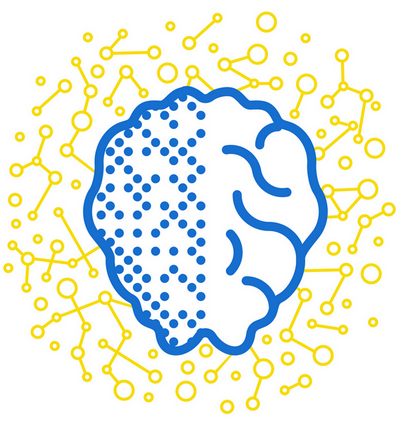
\includegraphics[height=1cm]{images/ipavlov-logo.png}}

\newcommand{\citepaper}[1]{\citetitle{#1} by \citeauthor{#1}}

%\graphicspath{{./images}}

%\usetheme{lucid}
\begin{document}

\begin{frame}
    \titlepage
\end{frame}

%\begin{frame}
%\frametitle{Overview}
%
%\begin{itemize}
%    \item Does unsupervised representation learning for images
%    \item An ambiguous
%\end{itemize}
%
%\end{frame}

\begin{frame}
\frametitle{How to estimate mutual information (MI) with neural networks?}

\begin{itemize}
    \item\pause Imagine we have two random variables $X$ and $Y = E(X)$, where $Y$ is obtained by encoding $X$ via $E(.)$.
    \item\pause By Donsker-Varadhan inequality for any function $f$ we have:
\begin{equation*}
I(X; Y) \triangleq \kl{p(x,y)}{p(x)p(y)} \geq \expect[p(x,y)]{f(x,y)} - \log \expect[p(x)p(y)]{e^{f(x,y)}}
\end{equation*}

    \item\pause This looks like a discriminator!
    \item\pause Let's train a discriminator $T_\omega$ to maximize:
\begin{equation*}
\expect[p(x,y)]{T_\omega(x,y)} - \log \expect[p(x)p(y)]{e^{T_\omega(x,y)}}
\end{equation*}
    \item\pause I.e. $T_\omega$ is trained to distinguish between paired examples $(x, E(x))$ and unpaired examples $(x, y')$ (i.e. $y' \neq E(x)$).
    \item\pause If we did a good job in training $T_\omega$ then we'll have a good MI estimate between $X$ and $Y$.
\end{itemize}

\end{frame}

\begin{frame}
\frametitle{How to \textit{maximize} MI with neural networks?}

\begin{itemize}
    \item\pause Just use your discrminator $T_\omega$ to train an encoder $E_\psi$!
    \item\pause Updating an encoder will force use to retrain a discriminator $T_\omega$
    \item\pause Then let's train them in parallel, just like a GAN model!
    \item\pause It's exactly like a GAN model, but encoder $E_\psi$ \textit{helps} discriminator $T_\omega$ instead of spoofing it since both try hard to increase the lower bound:
    \begin{itemize}
        \item\pause $T_\omega$ tries to increase LB to provide an accurate MI estimate.
        \item\pause $E_\psi$ tries to increase it because it will increase the MI
    \end{itemize}
\end{itemize}
\end{frame}

\begin{frame}
\frametitle{Global MI vs Local MI}

\begin{itemize}
    \item\pause Imagine we have a dataset of images $x_1, ..., x_n$ and an encoder $y = E_\psi(x)$.
    \item\pause Is it a reasonable objective to maximize $I(X, Y)$, i.e. MI between \textit{the whole} input and \textit{the whole} output?
    \item\pause No! Because a lot of information is irrelevant (for classification):
    \begin{figure}
        \centering
        \pause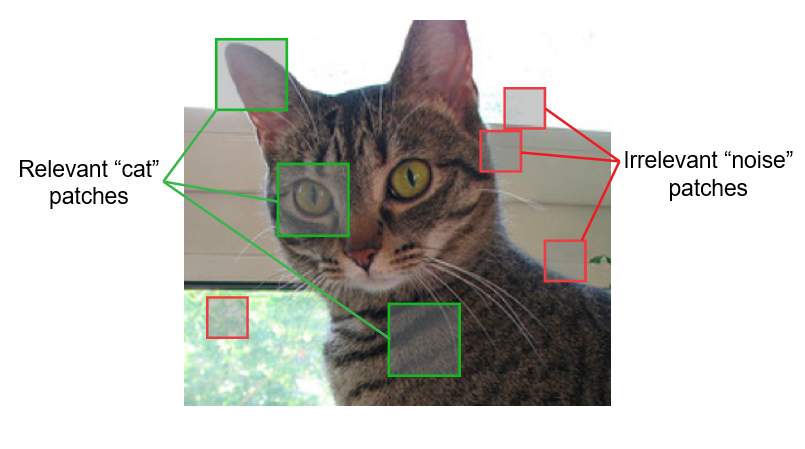
\includegraphics[width=0.8\textwidth]{images/cat-local-vs-global.png}
    \end{figure}
    \item\pause Let's maximize MI between local patches and the output then!
\end{itemize}

\end{frame}

\begin{frame}
\frametitle{Deep InfoMax with \textit{global} objective}

\begin{itemize}
    \item\pause Pre-encode an image into 3d-tensor $c = C_\psi(x)$ of ``local'' feature vectors.
    \item\pause Compute a ``global'' feature vector $y = E_\psi(c)$ (by avg-pooling followed by MLP, for example).
    \item\pause Train $T_\omega, C_\psi, E_\psi$ to maximize $I(c, y)$.
    \item\pause I.e. our $T_\omega$ takes $c$ and $y$ as inputs and outputs a scalar score.
\end{itemize}

\pause
\begin{figure}
\centering
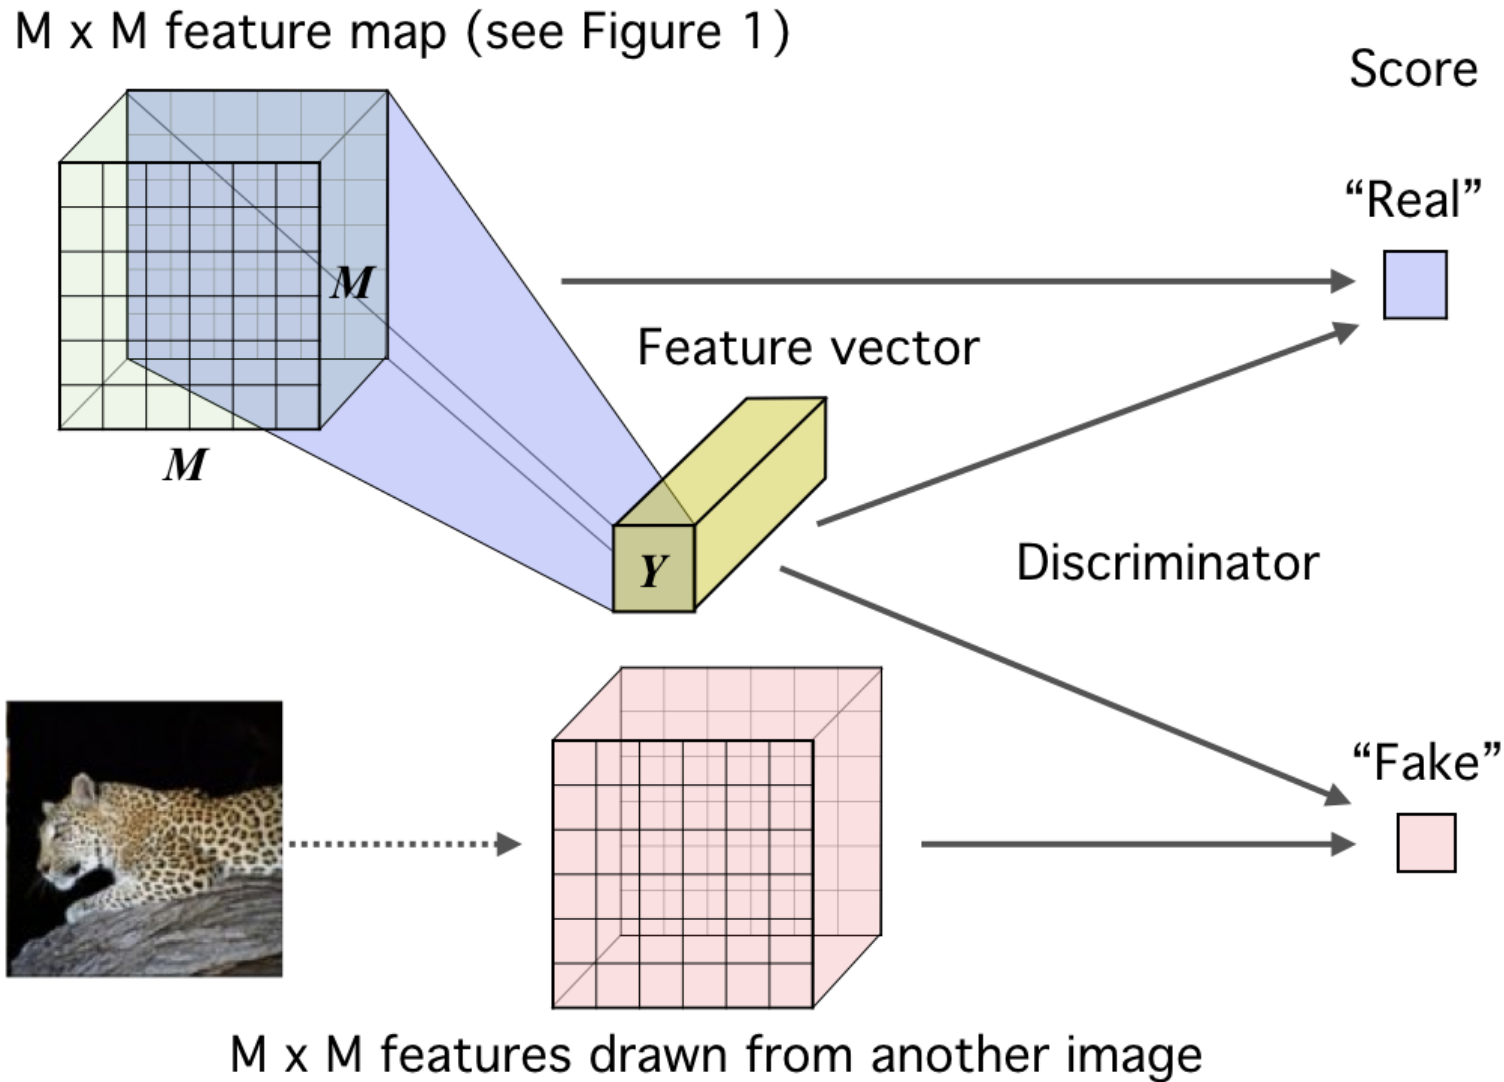
\includegraphics[width=0.7\textwidth]{images/dim_global.png}
\end{figure}

\end{frame}

\begin{frame}
\frametitle{Deep InfoMax with \textit{local} objective}
\begin{itemize}
    \item\pause Do the same as for the global objective, but split $c$ into local features and maximize:
    \begin{equation*}
    \frac{1}{M^2}\sum_{i,j}I(c_{i,j}(x), y)
    \end{equation*}
    \item\pause I.e. we maximize the MIs between local patches and a global vector.
    \item\pause This forces the model to encode useful global information.
\end{itemize}

\pause
\begin{figure}
\centering
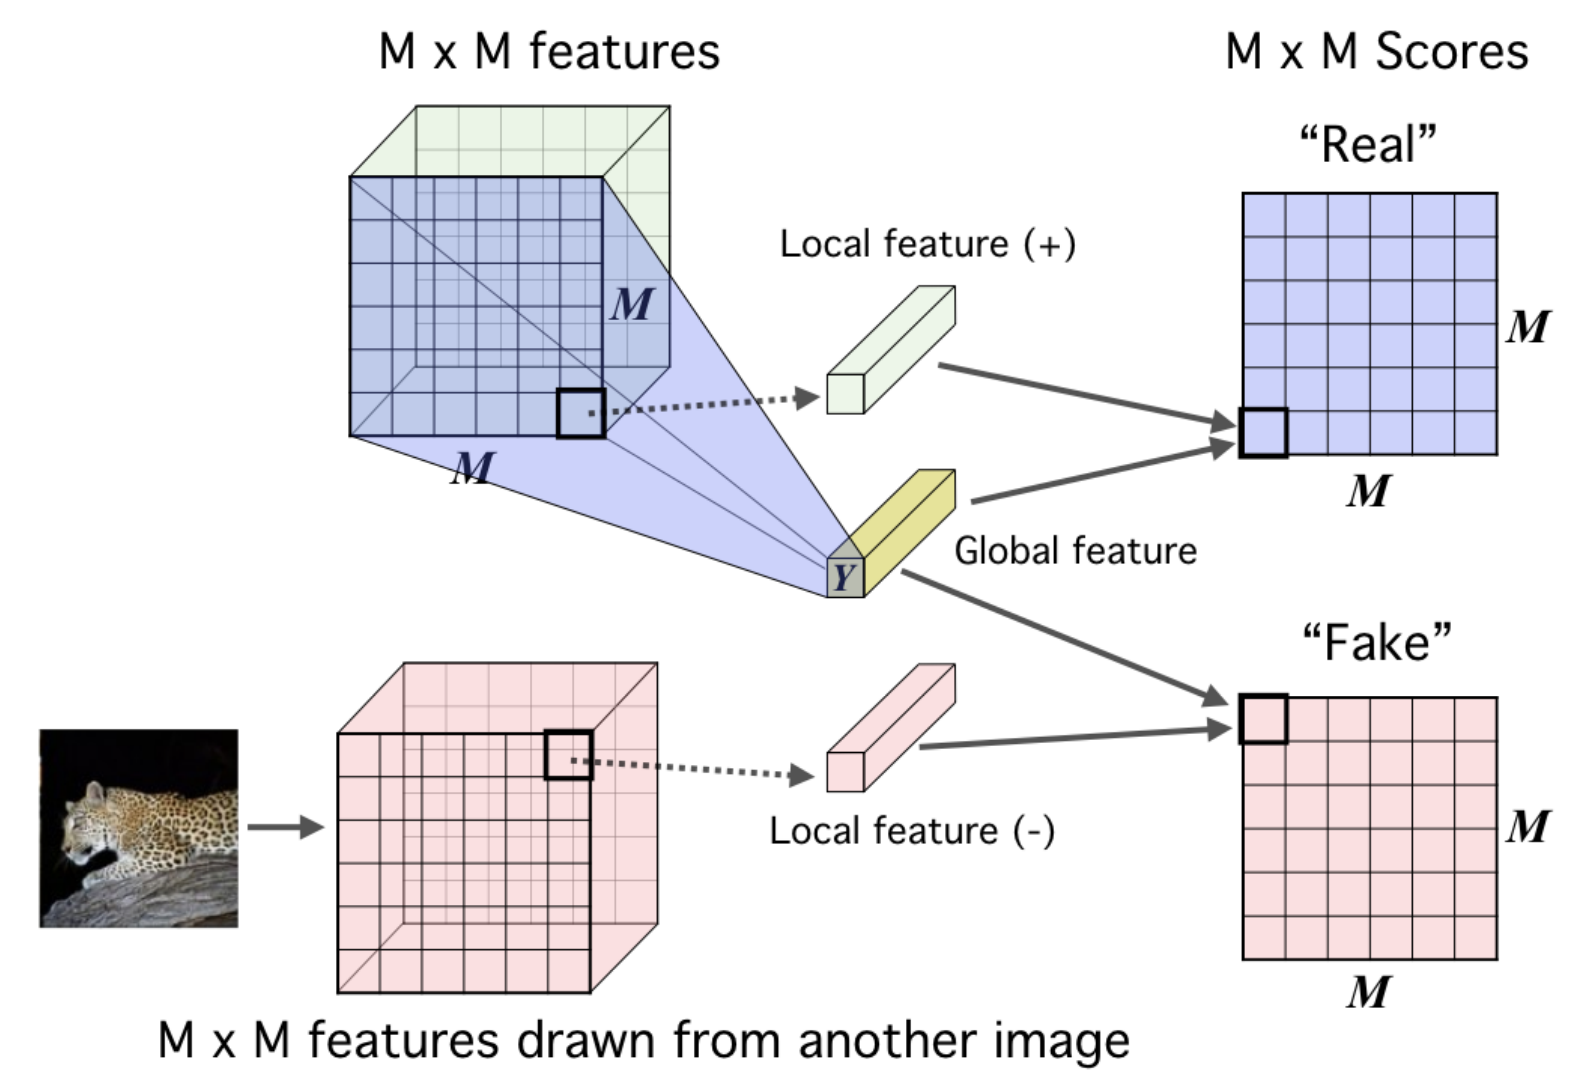
\includegraphics[width=0.7\textwidth]{images/dim_local.png}
\end{figure}

\end{frame}


\begin{frame}
\frametitle{Some details and thoughts}

\begin{itemize}
    \item\pause In practice we combine both the global and local objectives during training.
    \item\pause We also need to regularize the representations to be similar to some simple prior distribution.
    \item\pause They conduct \textbf{a ton of} experiments on different datasets and for different downstream tasks demonstraing SotA results.
    \item\pause There are some different variants on how to reformulate the LB to make the training more stable.
    \item\pause There are some gritty details on how to do negative sampling properly.
    \item\pause The paper is written quite ambigously and a lot of important details are scattered all over the manuscript... (i.e. how we do summarization of $c$ into $y$, what prior do we use, etc)
\end{itemize}
\end{frame}


\end{document}
